\documentclass[11pt]{article}

\usepackage{a4wide}
\usepackage{mathptm}
\usepackage{xspace}
\usepackage{amsmath}
\usepackage{graphicx}
\usepackage{algorithm}
\usepackage{algpseudocode}
\usepackage{tikz}
\usepackage{tkz-graph}
\usetikzlibrary{shapes.misc, positioning}
\usepackage{listings}
\usepackage{color}
\usepackage{hyperref}

\definecolor{dkgreen}{rgb}{0,0.6,0}
\definecolor{gray}{rgb}{0.5,0.5,0.5}
\definecolor{mauve}{rgb}{0.58,0,0.82}

\lstset{frame=tb,
  language=Java,
  aboveskip=3mm,
  belowskip=3mm,
  showstringspaces=false,
  columns=flexible,
  basicstyle={\small\ttfamily},
  numbers=left,
  numberstyle=\tiny\color{gray},
  keywordstyle=\color{blue},
  commentstyle=\color{dkgreen},
  stringstyle=\color{mauve},
  breaklines=true,
  breakatwhitespace=true,
  tabsize=3
}
\begin{document}

\title{My Best Software Technology Evaluation Project Ever}

\author{Some Student and Some other Student}

\maketitle

\begin{abstract}

  10-15 lines with the software technology and the highlights from the
  project that has been undertaken.

\end{abstract}

%\input{commands}


\section{Introduction}

\label{sec:introduction}

In this project, our task is to study specific software development technologies and platforms. Specifically, we will:

\begin{itemize}
    \item Complete a FeedApp prototype implementation with free choice of technology stack
    \item Implement a new technology in our stack and perform a technology assessment
\end{itemize}

\subsection{Prototype implementation}

Our prototype is an implementation of a polling application. Users can create, vote on, and delete polls. The application includes a nice front-end, where potential users have to create accounts to use the application. 

\subsubsection{Implemented technology stack}

The technology stack we used was the following: 

\begin{itemize}
    \item Spring as the application framework
    \item React as the Web UI
    \item Redis for caching
    \item RabbitMQ for messaging
    \item JPA and H2 for persistence 
    \item Docker for containerization
    \item Github and Github Actions for the repository and CI
\end{itemize}

\subsection{Results}

Put results from the Neo4j experiment here

\begin{itemize}

\item A one paragraph overview at the end, explaining how the rest of the report is / has been organised.

\end{itemize}

\noindent
This rest of this report is organised as follows:
Section~\ref{sec:design} gives an overview of the functional aspects of the FeedApp application, information concerning the use cases, domain model and the architecture of the application. 
Put more overview here


\section{Design}
\label{sec:design}

Around 5 pages about functional aspects of the FeedApp application.

Concretely, you shall write about 

\begin{itemize}
	\item the \emph{use cases},
	\item the \emph{domain model}, and
	\item the \emph{architecture} (including applied technologies)
\end{itemize}

Each part shall ideally be accompanied with a graphical representation (diagram).

You may have a look at the \href{https://github.com/selabhvl/dat250public/blob/master/projectdescription/README.md}{Examples on GitHub}.



\section{Technology Assessment}
\label{sec:technology}


Introduce in (sufficient) depth the key concepts and architecture of the chosen software technology. As part if this, you may consider using a running example to introduce the technology.

This part and other parts of the report probably needs to refer to
figures. Figure~\ref{fig:framework} from \cite{brown:96} just
illustrates how figure can be included in the report.

\begin{figure}[thb]
	\centering
	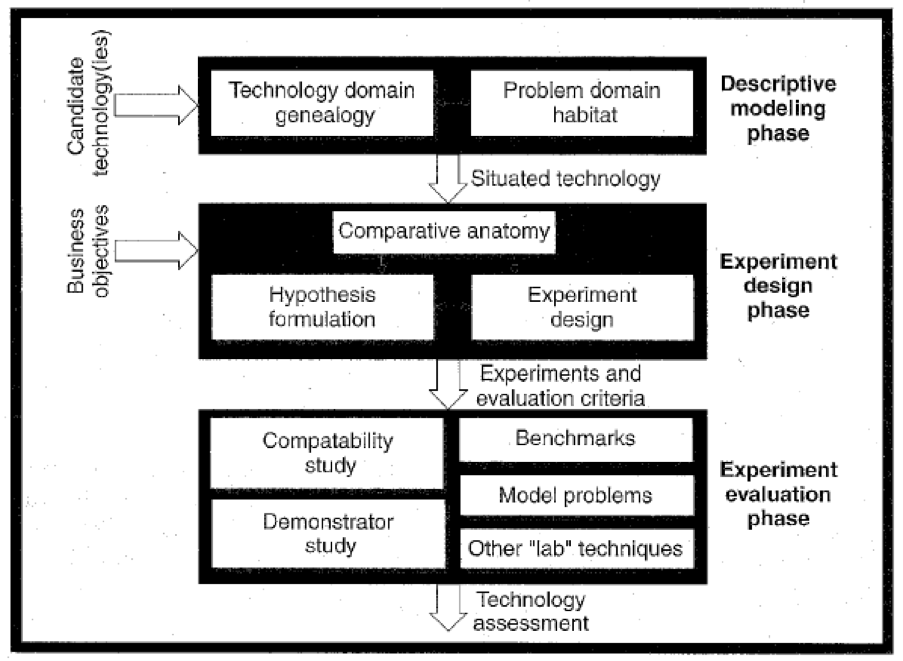
\includegraphics[scale=0.5]{figs/framework.png}
	\caption{Software technology evaluation framework.}
	\label{fig:framework}
\end{figure}

\subsection{Descriptive Modeling}

write where the technology comes from, its history, its context and what problem it solves.
Consider drawing a graph like in \cite{brown:96}.

\subsection{Experiment Design}

Write you hypotheses about what benefits the technology bring and how you can support or reject them via experiments.

\subsection{Experiment Evaluation}

Write about the results of your experiments, either via personal experience reports, quantitative benchmarks, a demostrator case study or a combination of multiple approaches.


For some reports you may have to include a table with experimental
results are other kinds of tables that for instance compares
technologies. Table~\ref{tab:results} gives an example of how to create a table.

\begin{table}[bth]
	\centering
	\begin{tabular}{llrrrrrr}
		Config & Property & States & Edges & Peak & E-Time & C-Time & T-Time
		\\ \hline \hline
		22-2 & A   &    7,944  &   22,419  &  6.6  \%  &  7 ms & 42.9\% &  485.7\% \\
		22-2 & A   &    7,944  &   22,419  &  6.6  \%  &  7 ms & 42.9\% &  471.4\% \\
		30-2 & B   &   14,672  &   41,611  &  4.9  \%  & 14 ms & 42.9\% &  464.3\% \\
		30-2 & C   &   14,672  &   41,611  &  4.9  \%  & 15 ms & 40.0\% &  420.0\% \\ \hline
		10-3 & D   &   24,052  &   98,671  & 19.8  \%  & 35 ms & 31.4\% &  285.7\% \\
		10-3 & E   &   24,052  &   98,671  & 19.8  \%  & 35 ms & 34.3\% &  308.6\% \\
		\hline \hline
	\end{tabular}
	\caption{Selected experimental results on the communication protocol example.}
	\label{tab:results}
\end{table}



\section{Prototype Implementation}
\label{sec:implementation}

This section should provide brief details of how the prototype has been implemented.
You may want to use come code snippets here, but only focus on core features and aspects.
You are not meant to copy/paste your whole application code into the report.
Focus for instance how other developers may run your application and how they might develop it further...


The example below shows how you may include code. There are similar
styles for many other langages - in case you do not use Java in your
project. You can wrap the listing into a figure in case you need to
refer to it. How to create a figure was shown in Section~\ref{sec:technology}.

\lstinputlisting[language=java]{code/BoksVolum.java}



\section{Conclusions}

Concludes on the project, including the technology, its maturity,
learning curve, and quality of the documentation.

The references used throughput the report should constitute a well
chosen set of references, suitable for someone interesting in learning
about the technology.


\bibliographystyle{plain}
\bibliography{report.bib}{}

\end{document}
